\section{Admin}
\subsection{Hoàn thiện Dashboard}
\begin{figure}[H]
    \centering
    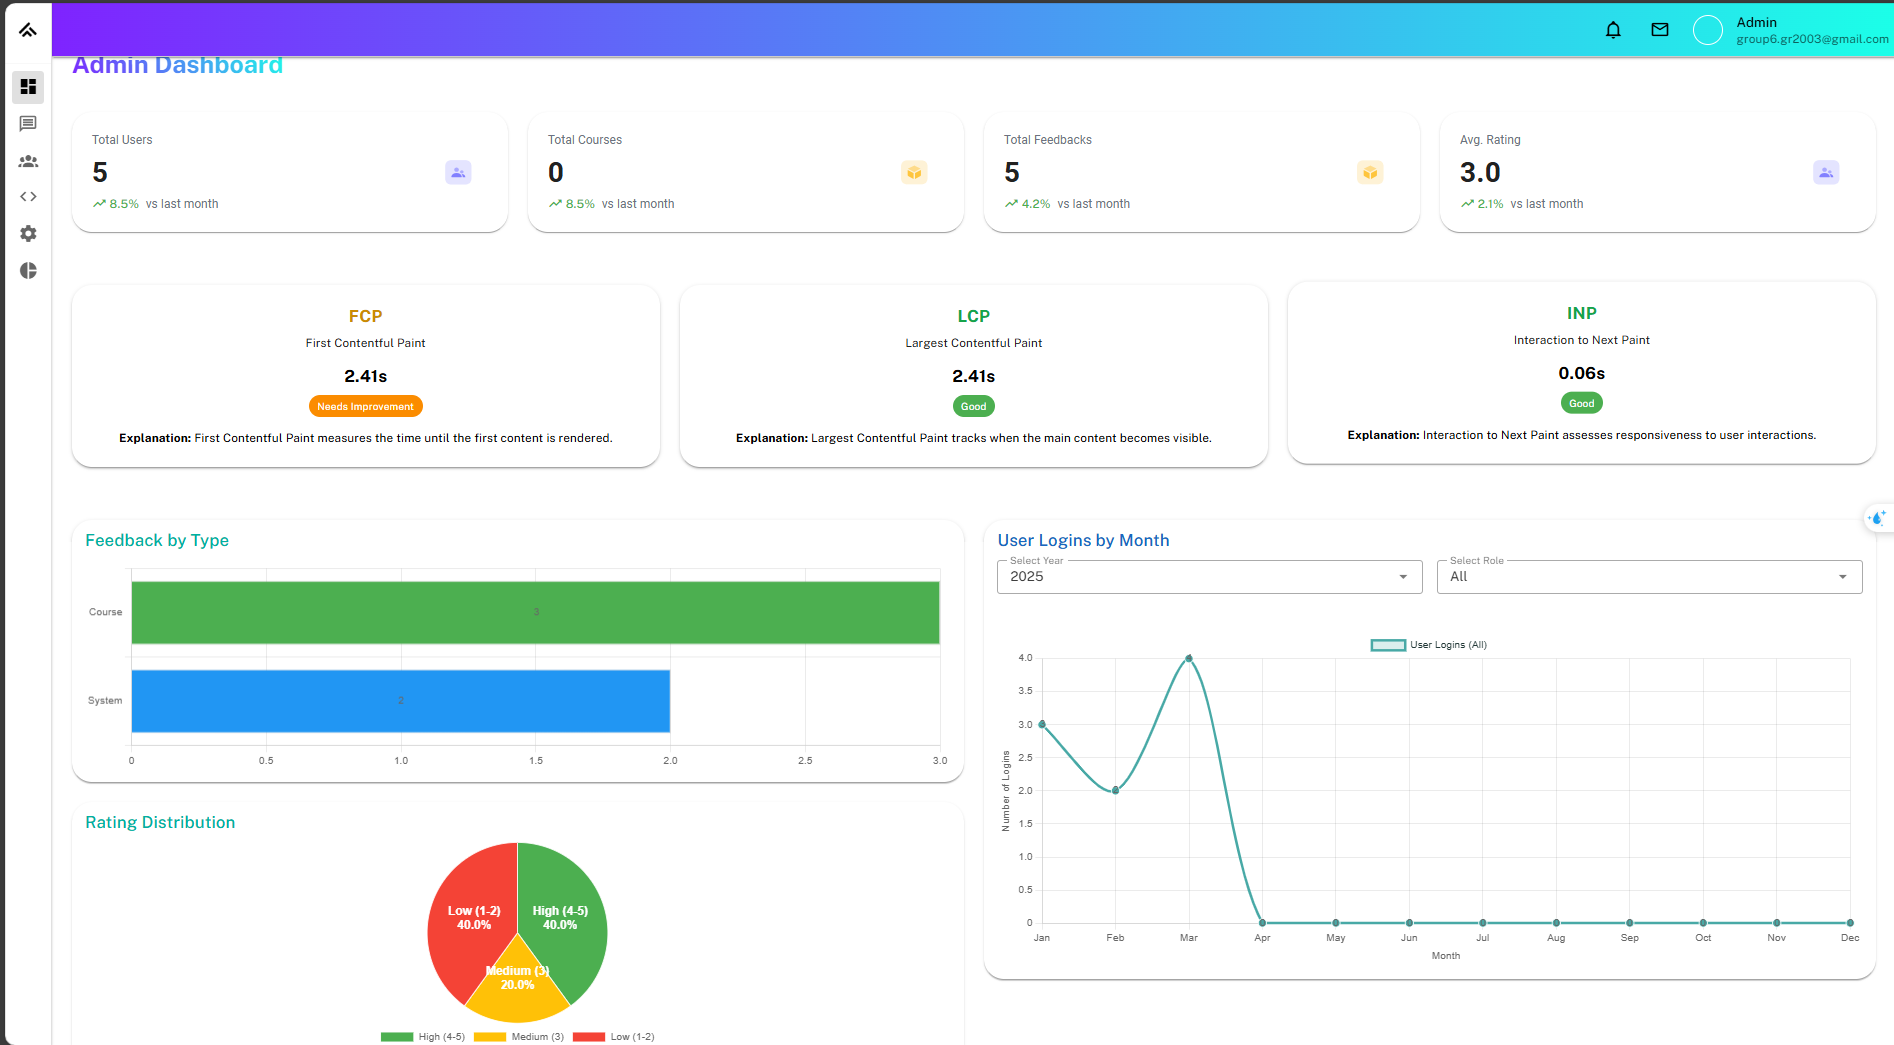
\includegraphics[width=0.8\linewidth]{images/admin_dashboard.png}
    \caption{Dashboard Admin}
    \label{fig:enter-label}
\end{figure}
Dashboard Admin, trang này như bảng điều khiển trung tâm để quản trị viên giám sát hệ thống. Nó hiển thị nổi bật các số liệu thống kê chính như:

\begin{itemize}
    \item Tổng số phản hồi gửi bởi người dùng.
    \item Tổng số người dùng đã đăng ký (bao gồm sinh viên, giáo viên và quản trị viên).
    \item Tổng số khóa học được cung cấp.
\end{itemize}

Các số liệu này cung cấp một cái nhìn tổng quan về hoạt động và mức độ tương tác của hệ thống. Dashboard tích hợp thêm biểu đồ để minh họa xu hướng theo thời gian, chẳng hạn như feedback hàng tuần hoặc sự tăng trưởng người dùng. 
\subsection{Quản lí các khóa học}
\begin{figure}[H]
    \centering
    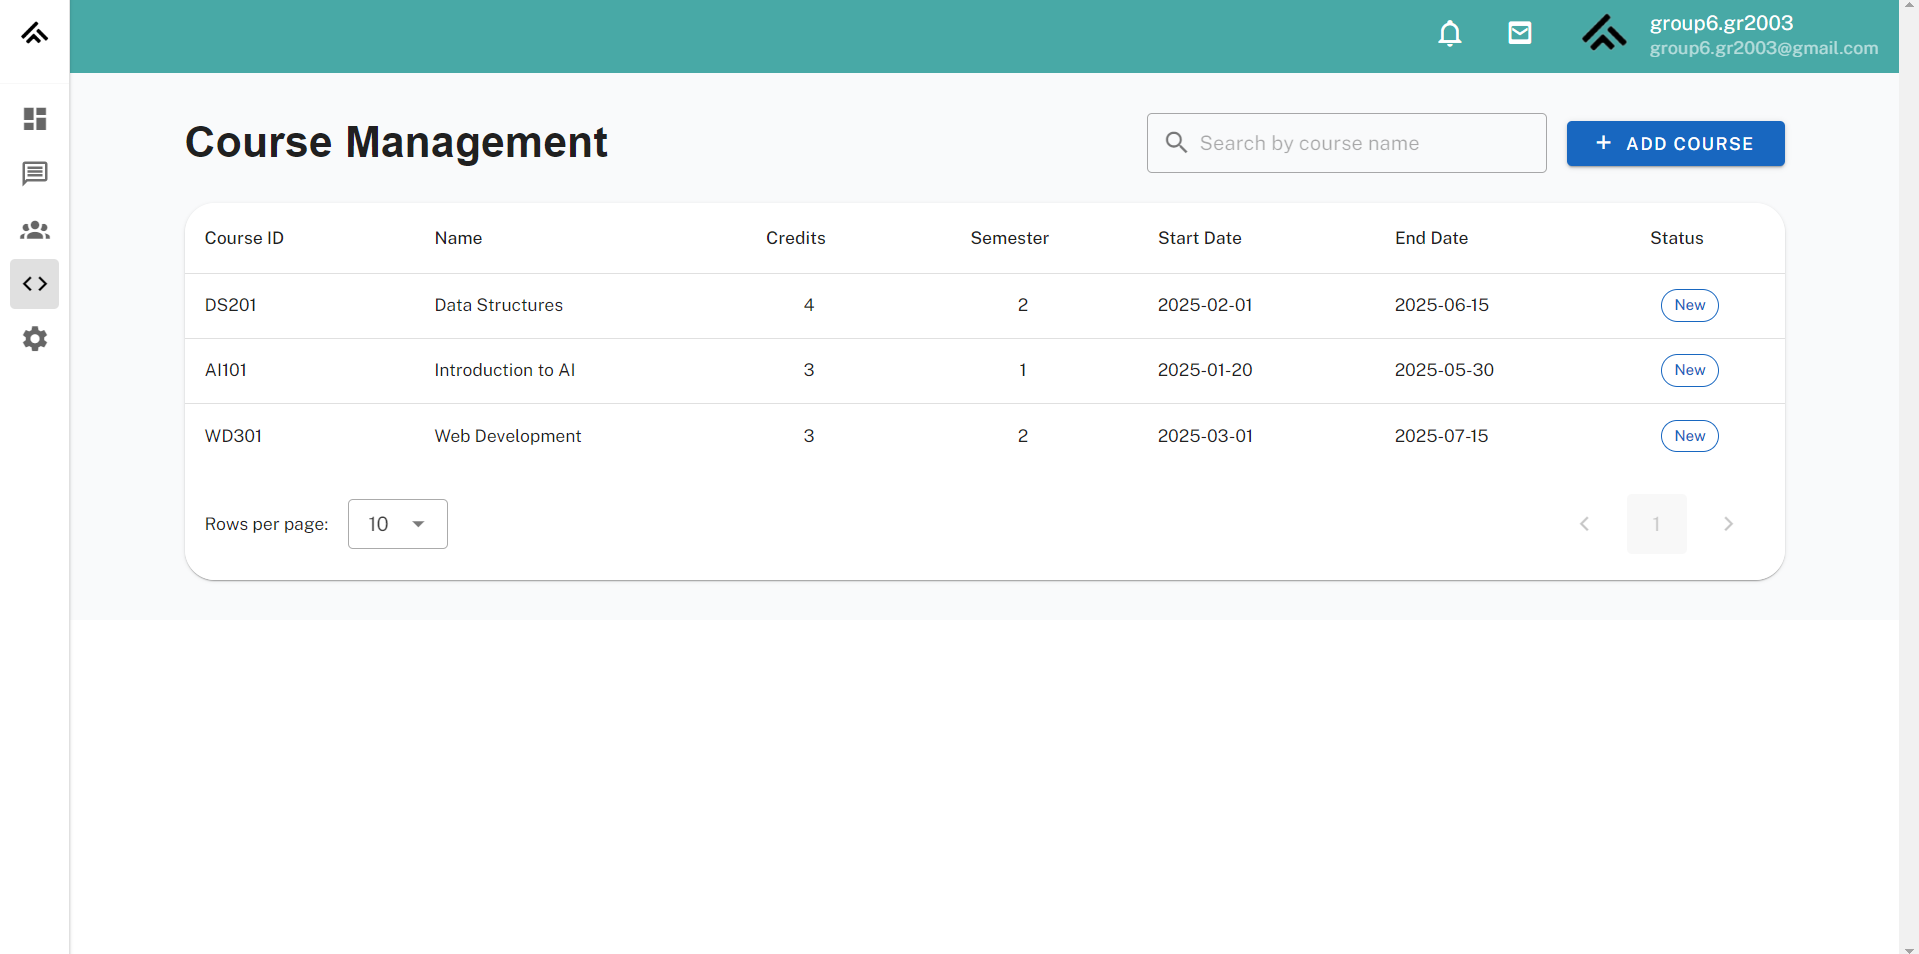
\includegraphics[width=0.8\linewidth]{images/admin_course_management.png}
    \caption{Quản lí danh sách khóa học của hệ thống}
    \label{fig:enter-label}
\end{figure}
Giao diện cung cấp một danh sách các khóa học với các cột chi tiết như:
\begin{itemize}
    \item Tiêu đề khóa học.
    \item Giáo viên, sinh viên được chỉ định.
    \item Số tín chỉ, học kì.
\end{itemize}

Quản trị viên có thể:
\begin{itemize}
    \item Chỉnh sửa chi tiết khóa học.
    \item Thêm khóa học mới.
    \item Xóa các khóa học.
\end{itemize}

\subsection{Thêm khóa học}
\begin{figure}[H]
    \centering
    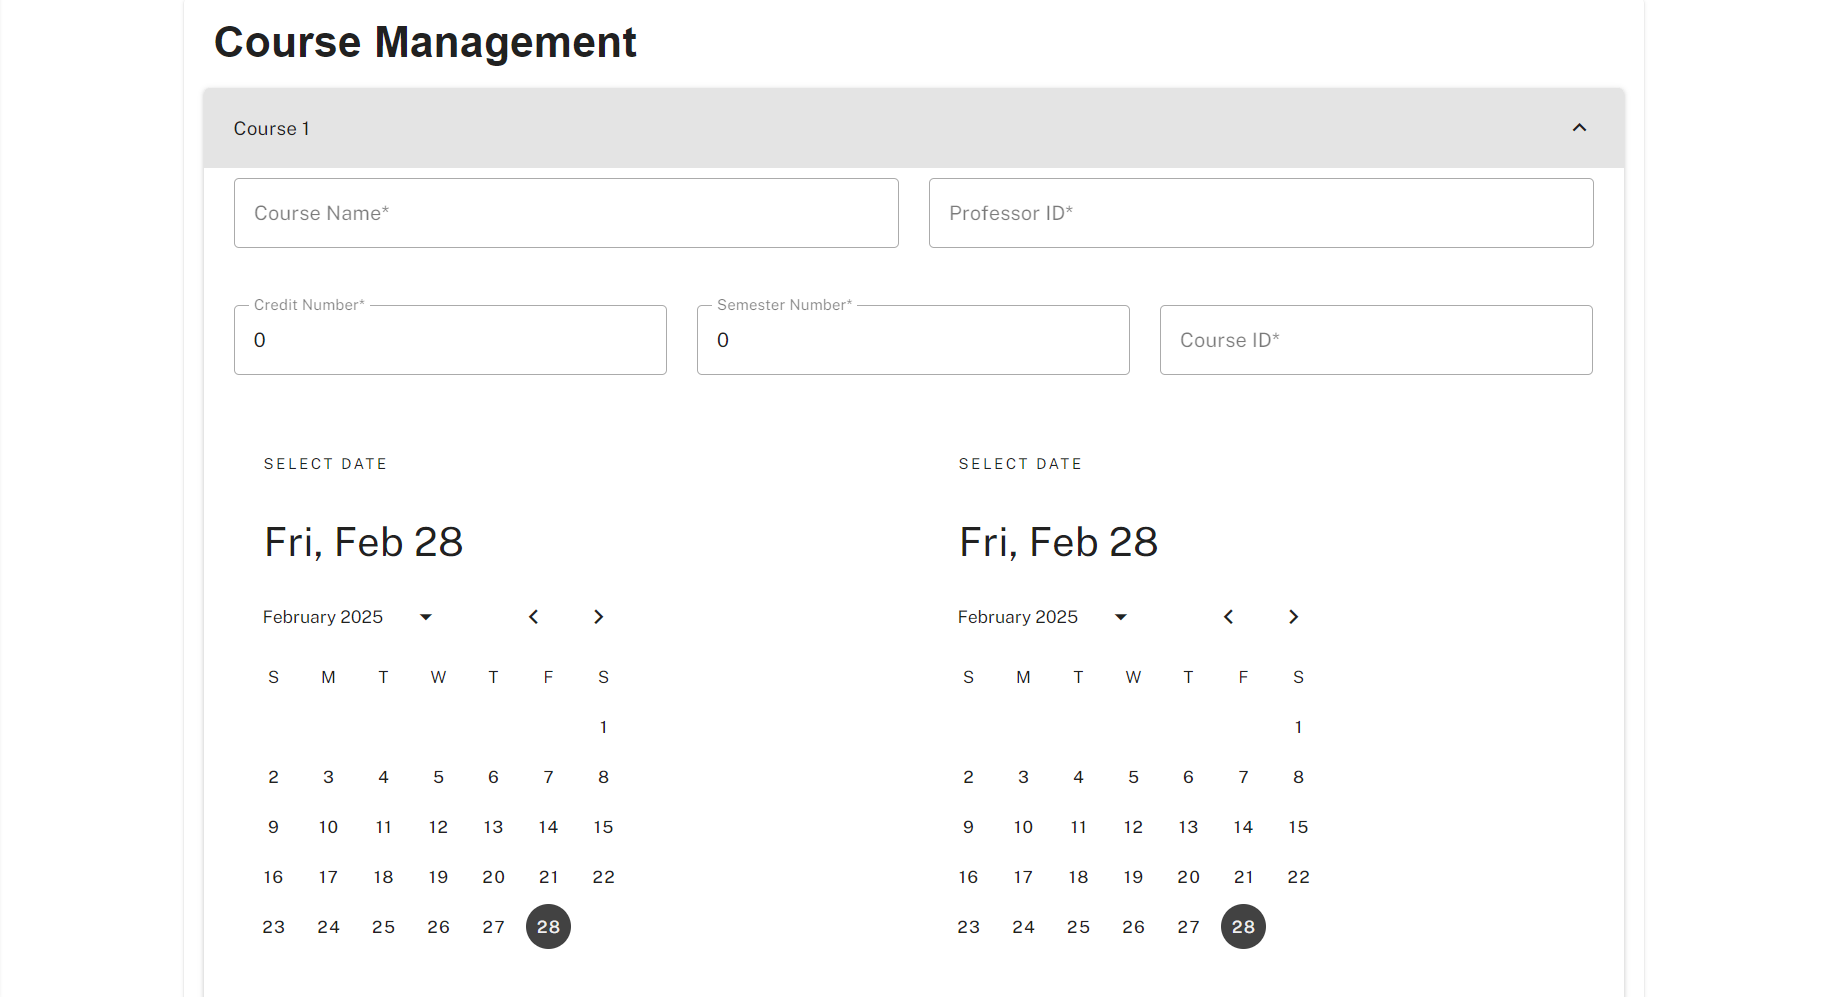
\includegraphics[width=0.8\linewidth]{images/admin_add_detail_course.png}
    \caption{Thông tin chi tiết khi thêm một khóa học}
    \label{fig:enter-label}
\end{figure}
Modal thêm khóa học bao gồm;
\begin{itemize}
    \item Tên khóa học: Mã định danh duy nhất.
    \item Mô tả khóa học: Tóm tắt mục tiêu và nội dung.
    \item Chỉ định giáo viên: ID của giáo viên phụ trách.
    \item Số tín chỉ, số học kì, thời gian khóa học
    \item Danh sách sinh viên
\end{itemize}
\begin{figure}[H]
    \centering
    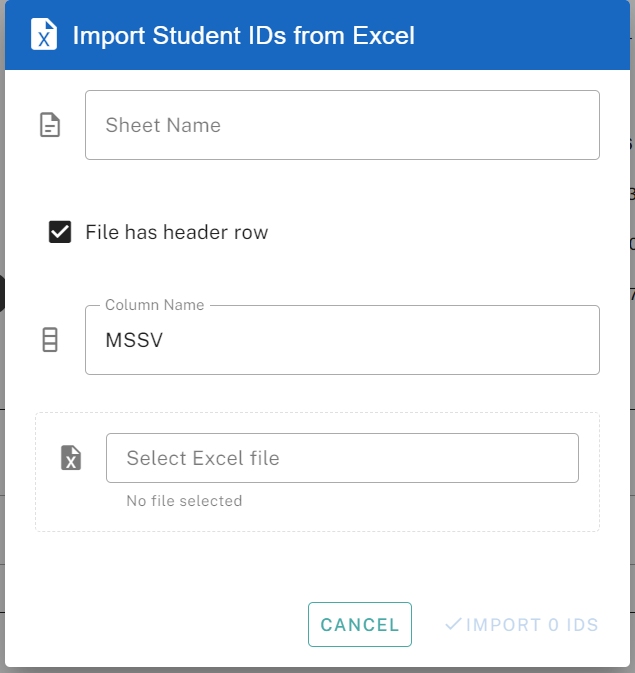
\includegraphics[width=0.6\linewidth]{images/admin_import_student_in_course.png}
    \caption{Thêm danh sách sinh viên vào khóa học}
    \label{fig:enter-label}
\end{figure}
Quá trình ghi danh sinh viên vào khóa học bằng cách nhập mã số từ tệp Excel. Tính năng này tối ưu hóa hiệu quả, đặc biệt với nhóm lớn. Giao diện cho phép:
\begin{itemize}
    \item Tải lên bảng Excel chứa mã số sinh viên (MSSV), tên, và có thể thêm email.
    \item Xác nhận tên sheet hoặc hàng tiêu đề để trích xuất dữ liệu chính xác.
\end{itemize}
So với nhập thủ công, quá trình này tiết kiệm thời gian và công sức, lý tưởng cho ghi danh hàng loạt vào đầu học kỳ hoặc chương trình đào tạo.
\begin{figure}[H]
    \centering
    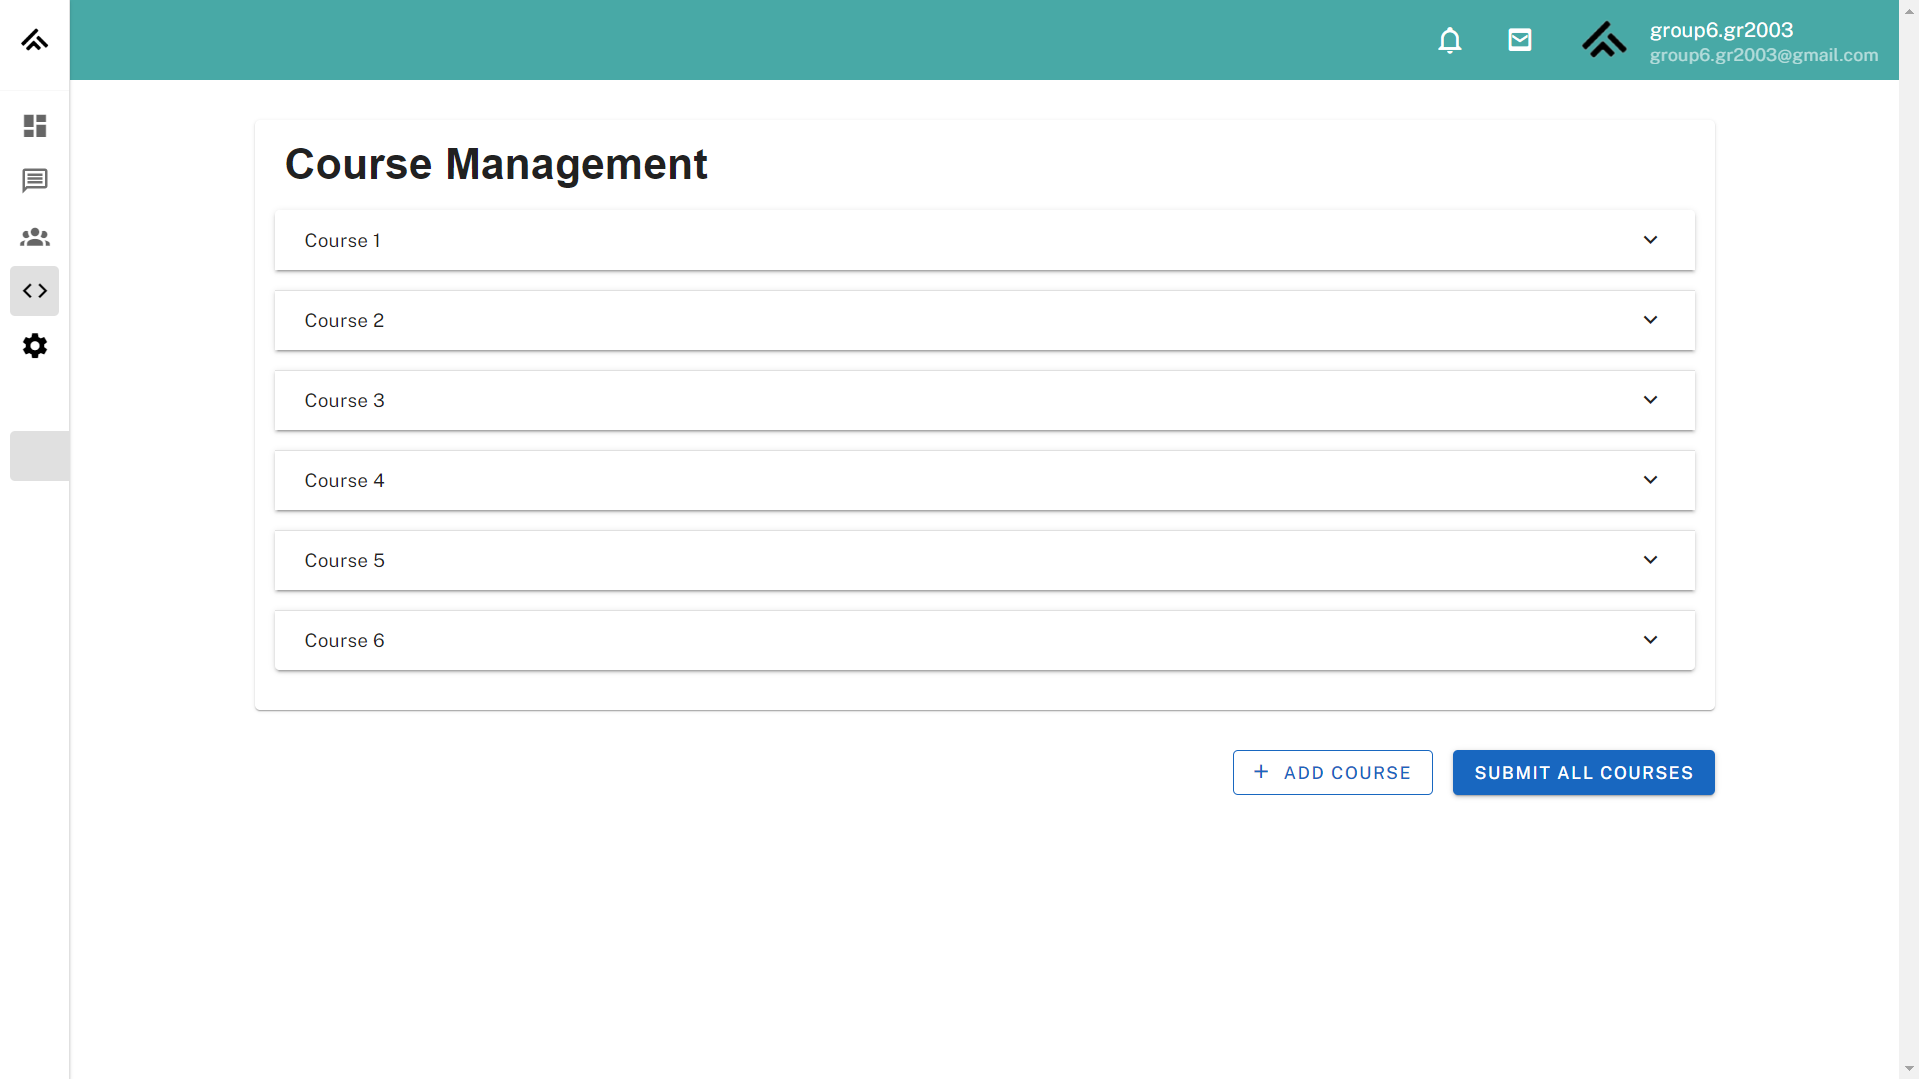
\includegraphics[width=0.6\linewidth]{images/admin_add_courses.png}
    \caption{Thêm nhiều khóa học}
    \label{fig:enter-label}
\end{figure}

Admin có thể thêm nhiều khóa học cùng một lúc.
\subsection{Thêm người dùng}
\begin{figure}[H]
    \centering
    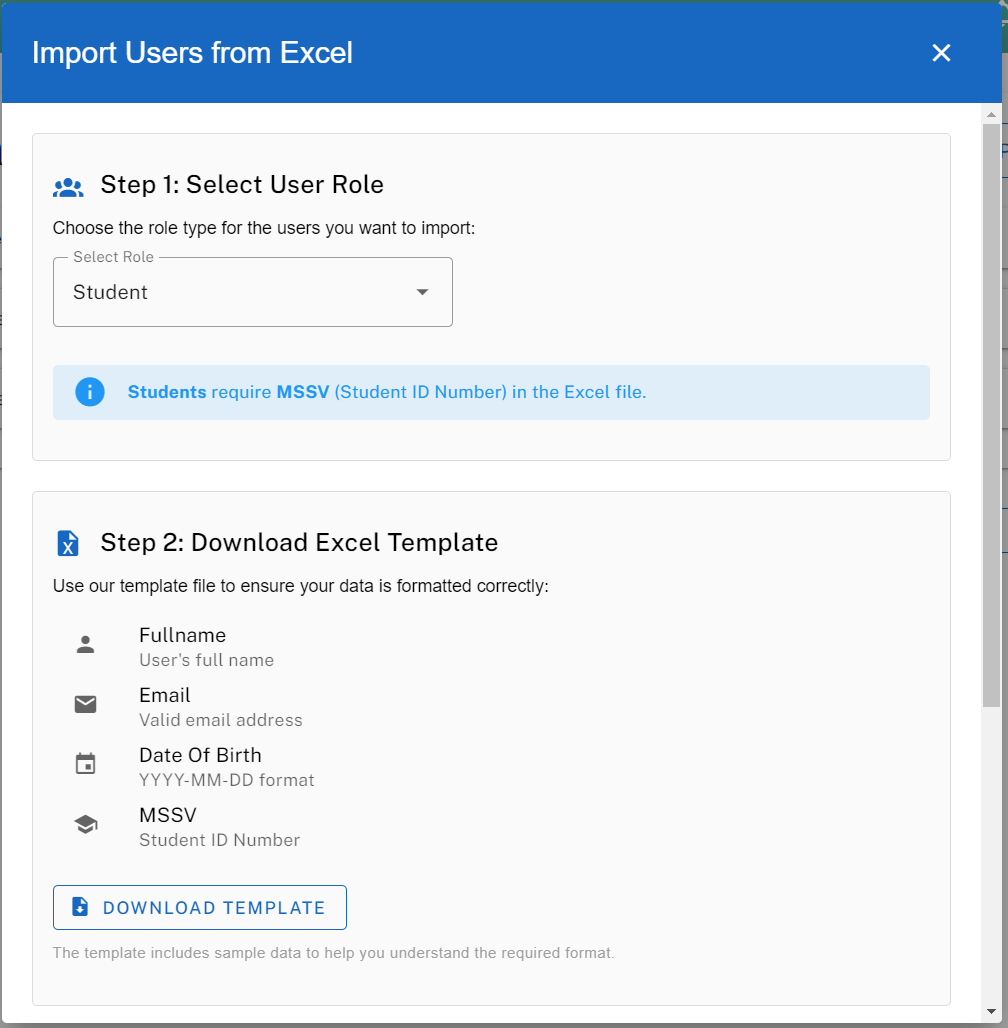
\includegraphics[width=0.6\linewidth]{images/admin_add_user_1.png}
    \caption{Thêm người dùng vào hệ thống }
    \label{fig:enter-label}
\end{figure}
\begin{figure}[H]
    \centering
    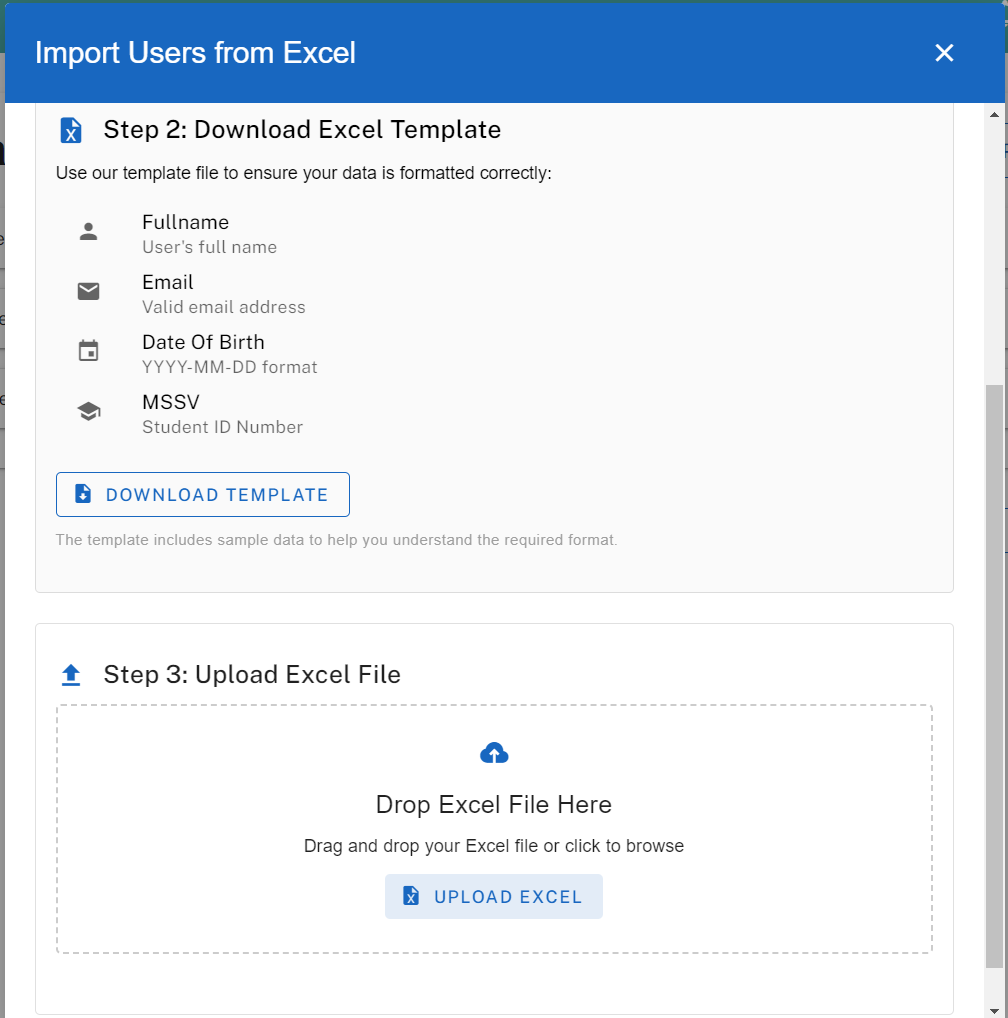
\includegraphics[width=0.6\linewidth]{images/admin_add_user_2.png}
    \caption{Caption}
    \label{fig:enter-label}
\end{figure}
Giao diện thêm người dùng mới (sinh viên, giáo viên, hoặc quản trị viên) vào nền tảng. Quản trị viên có thể:
\begin{itemize}
    \item Nhập dữ liệu từ mẫu Excel với thông tin như tên, mã số (MSSV), email, và vai trò.
    \item Cài đặt quyền theo vai trò (ví dụ: giáo viên tạo khóa học, sinh viên chỉ học).
\end{itemize}
\section{Code Area}
\subsection{Sử dụng Judge0 API}
\begin{itemize}
    \item Judge0 API là một hệ thống thực thi mã nguồn trực tuyến mã nguồn mở tiên tiến, được thiết kế để mạnh mẽ và có khả năng mở rộng. Đây là một công cụ cho phép thực hiện việc chạy mã nguồn trong nhiều ngôn ngữ lập trình khác nhau
    \item Điểm nổi bật của Judge0 là tính linh hoạt và khả năng tùy chỉnh. Judge0 API cho phép tùy chọn biên dịch, thêm đối số dòng lệnh, hoặc đặt giới hạn về thời gian và bộ nhớ khi thực thi mã nguồn. Điều này đặc biệt quan trọng nếu bạn dùng Judge0 trong các tác vụ đòi hỏi hiệu suất cao.
    \item Judge0 API hỗ trợ hơn 60 ngôn ngữ lập trình, từ những ngôn ngữ phổ biến mà bạn có thể đã sử dụng đến những ngôn ngữ ít gặp hơn.
\end{itemize}


\subsection{Thiết kế chức năng cho student làm bài tập: code}
\begin{figure}[H]
    \centering
    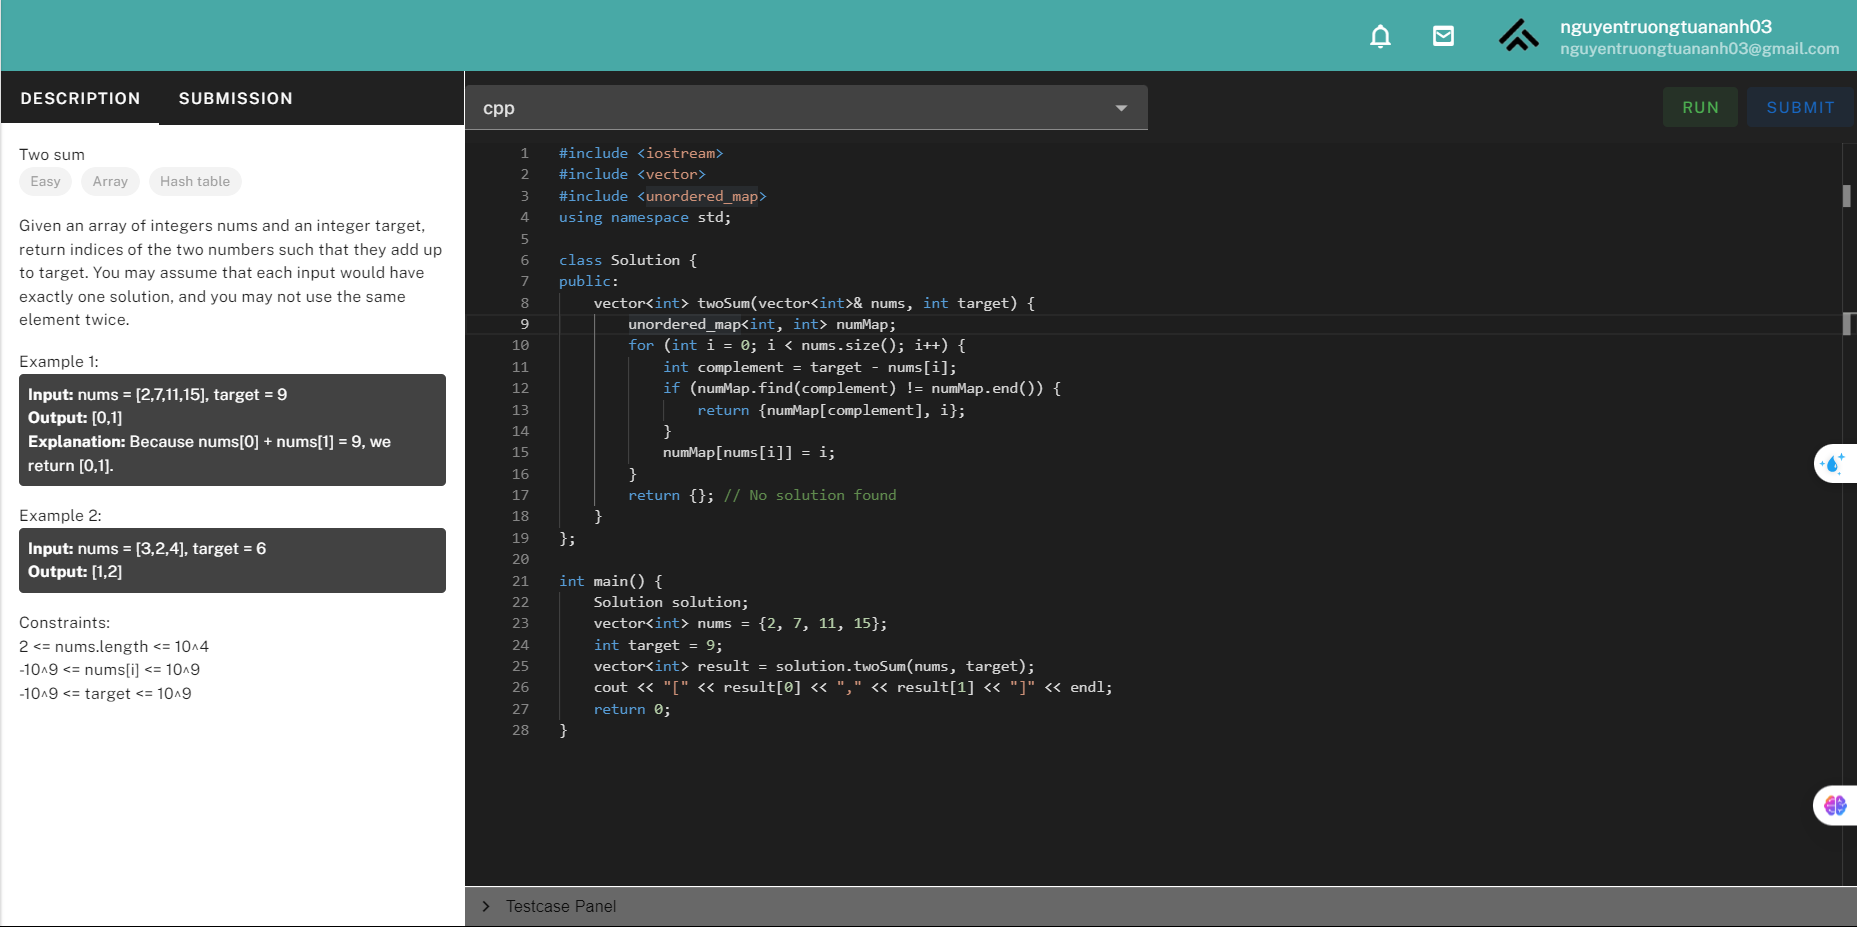
\includegraphics[width=0.8\linewidth]{images/code_area.png}
    \caption{Khu vực làm bài tập code}
    \label{fig:enter-label}
\end{figure}
Sinh viên có thể chọn ngôn ngữ lập trình, xem hướng dẫn, và truy cập mẫu đầu vào/đầu ra. Thiết lập này mô phỏng công cụ phát triển chuyên nghiệp, kết nối lý thuyết và thực hành. Tích hợp API Judge0 cung cấp đánh giá mã tự động, mang lại phản hồi tức thì để cải thiện kỹ năng học tập.
\begin{figure}[H]
    \centering
    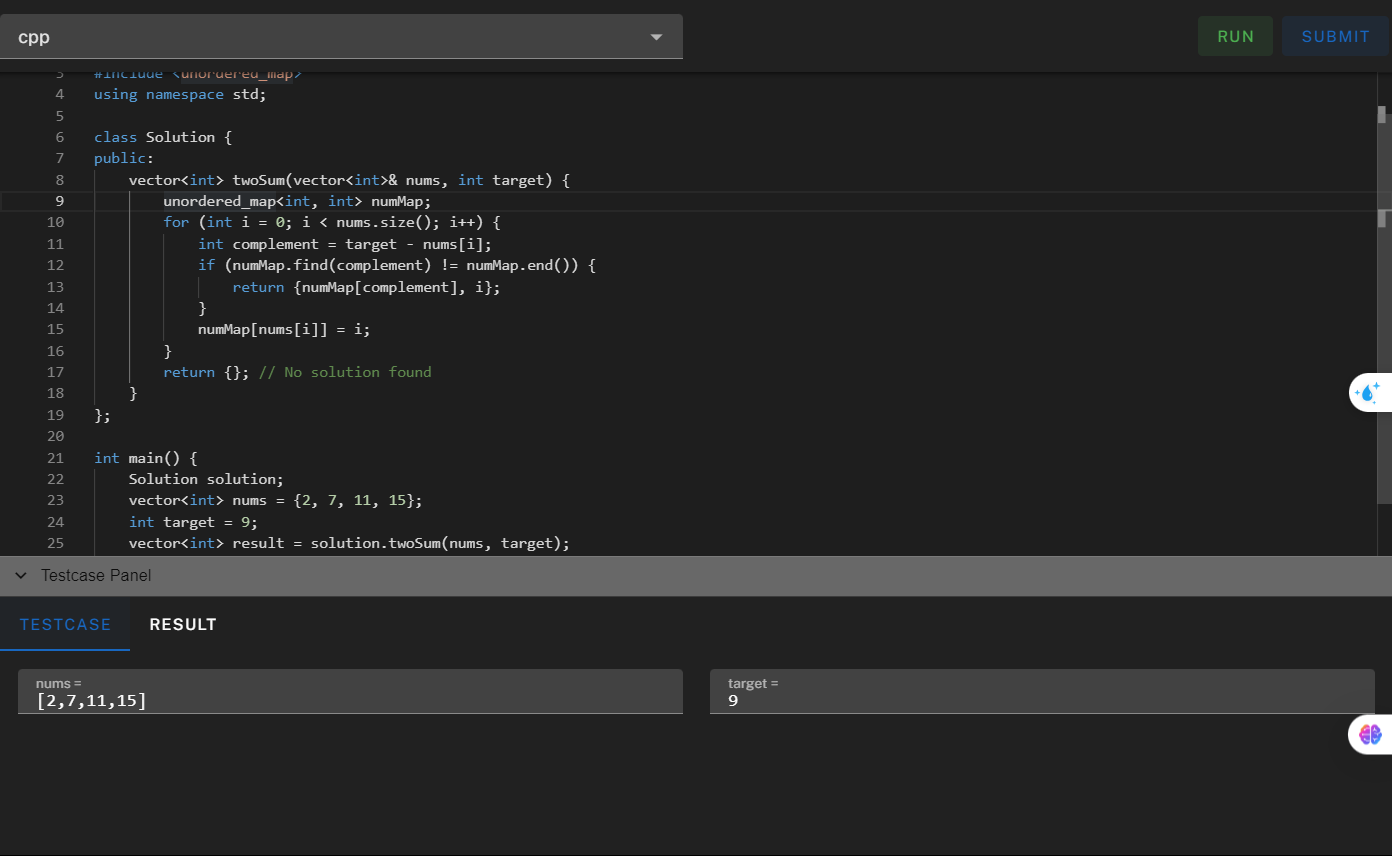
\includegraphics[width=0.8\linewidth]{images/code_testcase.png}
    \caption{Testcase bài tập}
    \label{fig:enter-label}
\end{figure}
Gaio diện hiển thị các testcase cho bài tập lập trình, cần thiết để đánh giá bài code của sinh viên. Mỗi trường hợp bao gồm:
\begin{itemize}
    \item Đầu vào cụ thể và đầu ra dự kiến.
    \item Một số hiển thị để hướng dẫn, một số ẩn để kiểm tra toàn diện.
\end{itemize}

\begin{figure}[H]
    \centering
    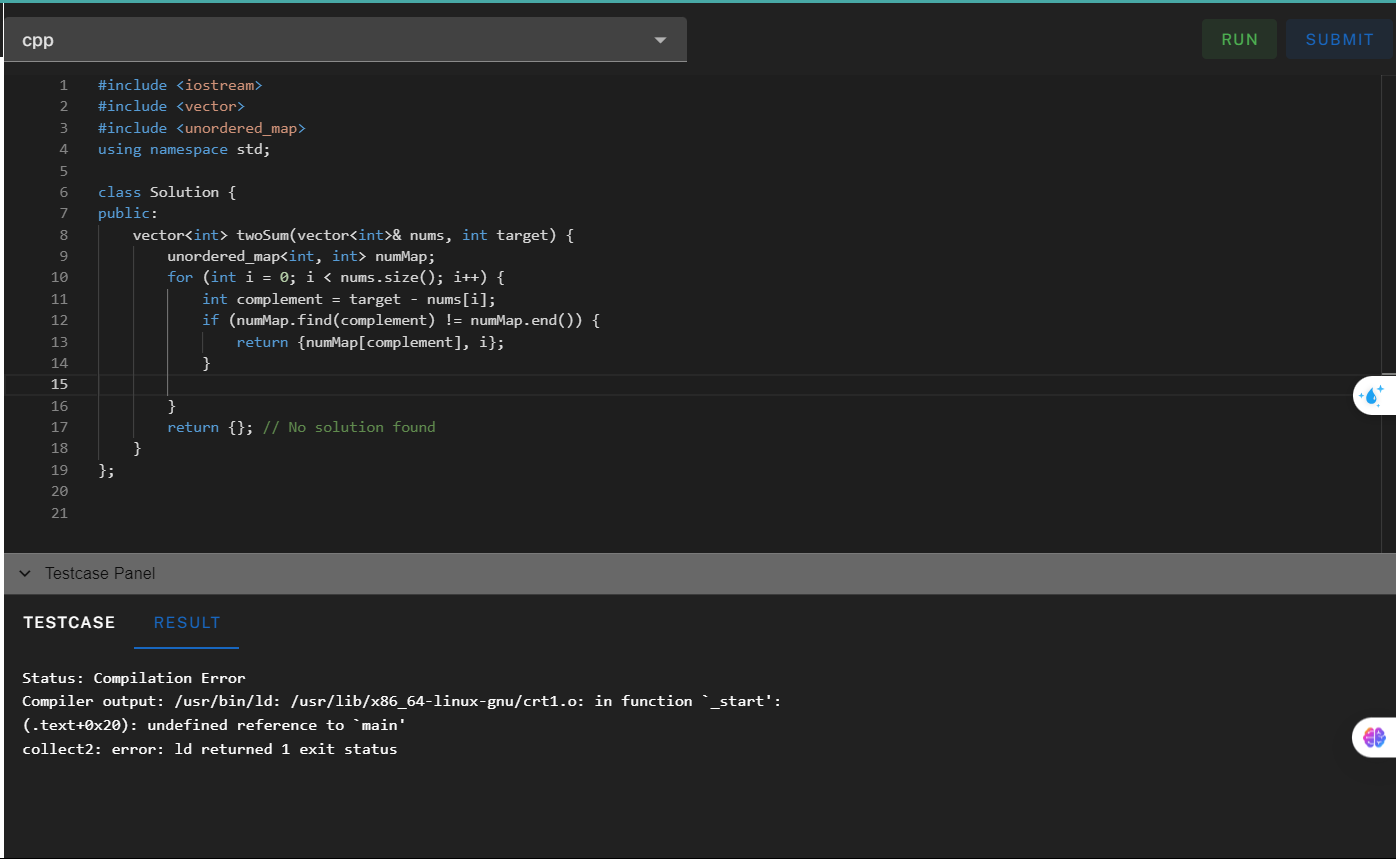
\includegraphics[width=0.8\linewidth]{images/code_run_error.png}
    \caption{Thông báo kết quả khi code chạy lỗi}
    \label{fig:enter-label}
\end{figure}
Kết quả thông báo lỗi khi đoạn code sinh viên lỗi
\begin{itemize}
    \item Loại lỗi: Cú pháp, thời gian chạy, v.v.
    \item Số dòng: Vị trí lỗi.
    \item Phản hồi chi tiết giúp sinh viên xác định sai lầm, hiểu nguyên nhân, và học hỏi.
\end{itemize}
\begin{figure}[H]
    \centering
    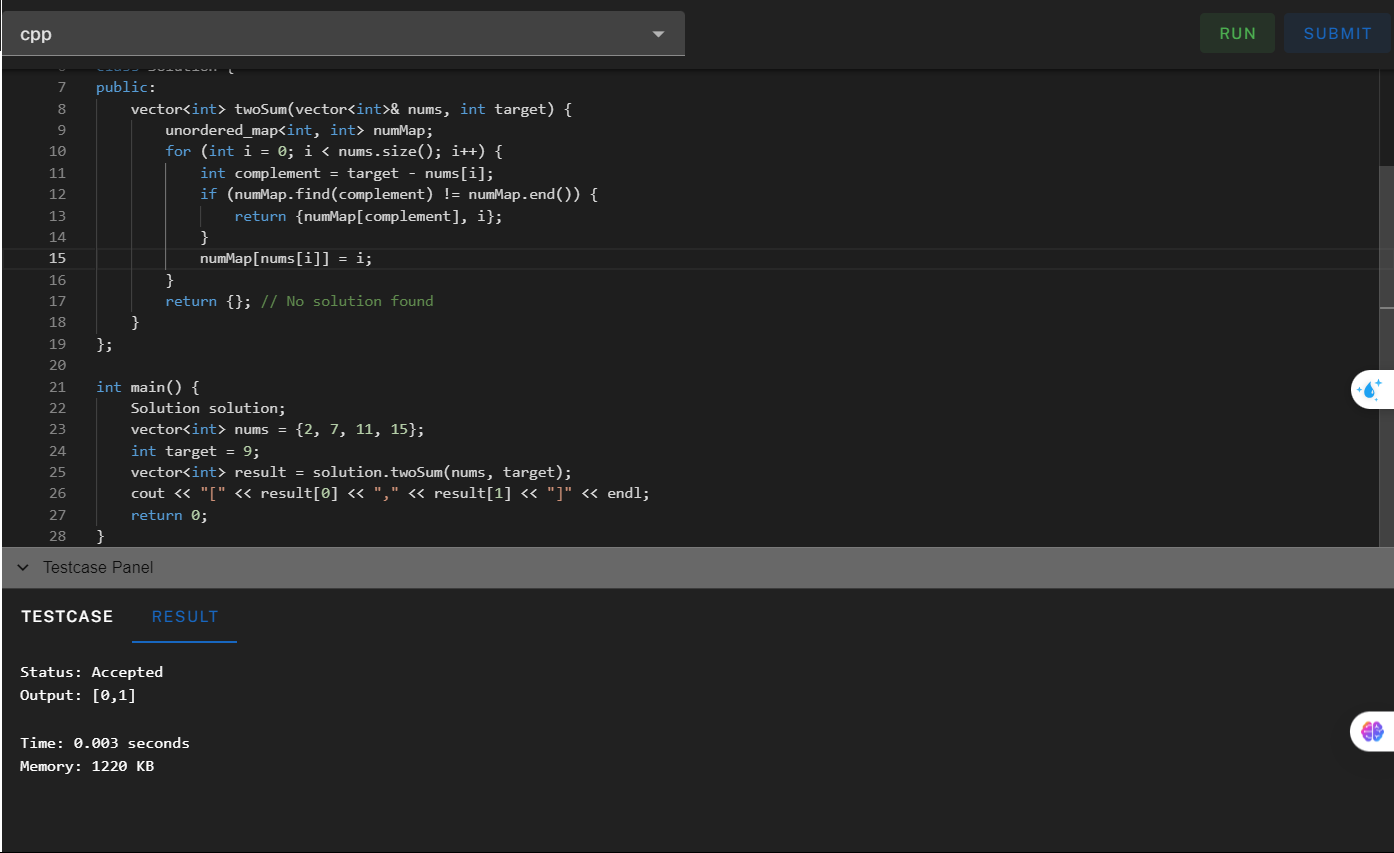
\includegraphics[width=0.8\linewidth]{images/code_run_success.png}
    \caption{Thông báo kết quả khi code chạy thành công}
    \label{fig:enter-label}
\end{figure}
Kết quả thông báo khi đoạn code sinh viên chạy thành công
\begin{itemize}
    \item Số trường hợp kiểm thử đã qua.
    \item Chỉ số hiệu suất (thời gian thực thi, bộ nhớ).
    \item Thông báo này củng cố tích cực, cung cấp cái nhìn về hiệu quả mã.
\end{itemize}